\documentclass{article}
\usepackage{graphicx} % Required for inserting images
\usepackage{float}
\usepackage{listings}
\lstset{
    language=Python,
    basicstyle=\ttfamily\footnotesize,
    keywordstyle=\color{blue}\bfseries,
    commentstyle=\color{gray},
    stringstyle=\color{red},
    showstringspaces=false,
    numberstyle=\tiny\color{gray},
    frame=single,
    breaklines=true,
    captionpos=b,
}
\usepackage{xcolor}

\title{Introducción al Analisis de Datos: Ejercicio - Clase 3}

\author{Gabriel Freire Parola, Jonathan Suarez, Santiago Llugany, \\ Matias Cabello, Santiago Seleme}

\date{October 2025}

\begin{document}
\maketitle
\section*{UML}
\begin{figure}[H]
    \centering
    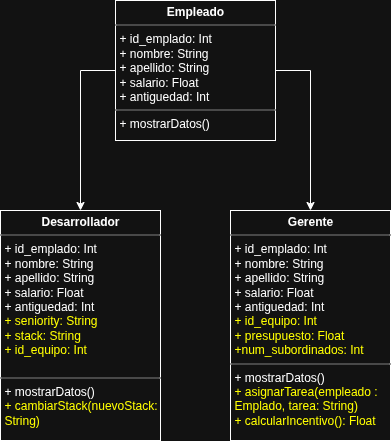
\includegraphics[width=0.75\linewidth]{diagrama_uml.png}
    \caption{Diagrama UML del sistema}
    \label{fig:placeholder}
\end{figure}
\section*{Script de Python}
\begin{lstlisting}[caption={Código python basado en el diagrama UML}, label={lst:python}]
# Clase base
class Empleado:
    def __init__(self, id_empleado: int, nombre: str, apellido: str, salario: float, antiguedad: int):
        self.id_empleado = id_empleado
        self.nombre = nombre
        self.apellido = apellido
        self.salario = salario
        self.antiguedad = antiguedad

    def mostrarDatos(self):
        print(f"ID: {self.id_empleado}")
        print(f"Nombre: {self.nombre} {self.apellido}")
        print(f"Salario: {self.salario}")
        print(f"Antigüedad: {self.antiguedad} años")


# Subclase: Desarrollador
class Desarrollador(Empleado):
    def __init__(self, id_empleado: int, nombre: str, apellido: str, salario: float, antiguedad: int,
                 seniority: str, stack: str, id_equipo: int):
        super().__init__(id_empleado, nombre, apellido, salario, antiguedad)
        self.seniority = seniority
        self.stack = stack
        self.id_equipo = id_equipo

    def mostrarDatos(self):
        super().mostrarDatos()
        print(f"Seniority: {self.seniority}")
        print(f"Stack: {self.stack}")
        print(f"ID de Equipo: {self.id_equipo}")

    def cambiarStack(self, nuevoStack: str):
        print(f"Cambiando stack de {self.stack} a {nuevoStack}")
        self.stack = nuevoStack


# Subclase: Gerente
class Gerente(Empleado):
    def __init__(self, id_empleado: int, nombre: str, apellido: str, salario: float, antiguedad: int,
                 id_equipo: int, presupuesto: float, num_subordinados: int):
        super().__init__(id_empleado, nombre, apellido, salario, antiguedad)
        self.id_equipo = id_equipo
        self.presupuesto = presupuesto
        self.num_subordinados = num_subordinados

    def mostrarDatos(self):
        super().mostrarDatos()
        print(f"ID de Equipo: {self.id_equipo}")
        print(f"Presupuesto: {self.presupuesto}")
        print(f"Número de subordinados: {self.num_subordinados}")

    def asignarTarea(self, empleado, tarea: str):
        print(f"{self.nombre} asigna la tarea '{tarea}' a {empleado.nombre}")

    def calcularIncentivo(self) -> float:
        incentivo = self.presupuesto * 0.05 + (self.num_subordinados * 100)
        print(f"Incentivo calculado: {incentivo}")
        return incentivo


# ===== Ejemplo de uso =====
if __name__ == "__main__":
    dev = Desarrollador(1, "Ana", "Pérez", 120000.0, 3, "Semi Senior", "Python/Django", 101)
    gerente = Gerente(2, "Luis", "Martínez", 200000.0, 5, 101, 500000.0, 8)

    print("\n=== Datos del Desarrollador ===")
    dev.mostrarDatos()

    print("\n=== Datos del Gerente ===")
    gerente.mostrarDatos()

    print("\n=== Ejemplo de interacción ===")
    gerente.asignarTarea(dev, "Actualizar API")
    gerente.calcularIncentivo()
    dev.cambiarStack("GoLang / React")
\end{lstlisting}
\end{document}
